\documentclass[
	%a4paper, % Use A4 paper size
	letterpaper, % Use US letter paper size
]{jdf}
\usepackage{graphicx}
\usepackage{biblatex}
\addbibresource{references.bib}


\author{Ali El-Khatib}
\email{aelkhatib6@gatech.edu}
\title{Homework 1}

\begin{document}
\maketitle
\section{Question 1}

\section{Question 2}
\subsection{General Data Protection Regulation & You}
The General Data Protection Regulation (GDPR) is a regulation regarding the protection of personal data and privacy, and adopted on April 27, 2016. In effect, it allows users within Europe to have increased control of all personal data (e.g., website cookies, email addresses, phone number)   The GDPR applies in both the European Union (EU) member states and the European Economic Area (EEA) illustrated in Figure~\ref{fig:europe-groups}. 
\begin{figure}
	\centering
	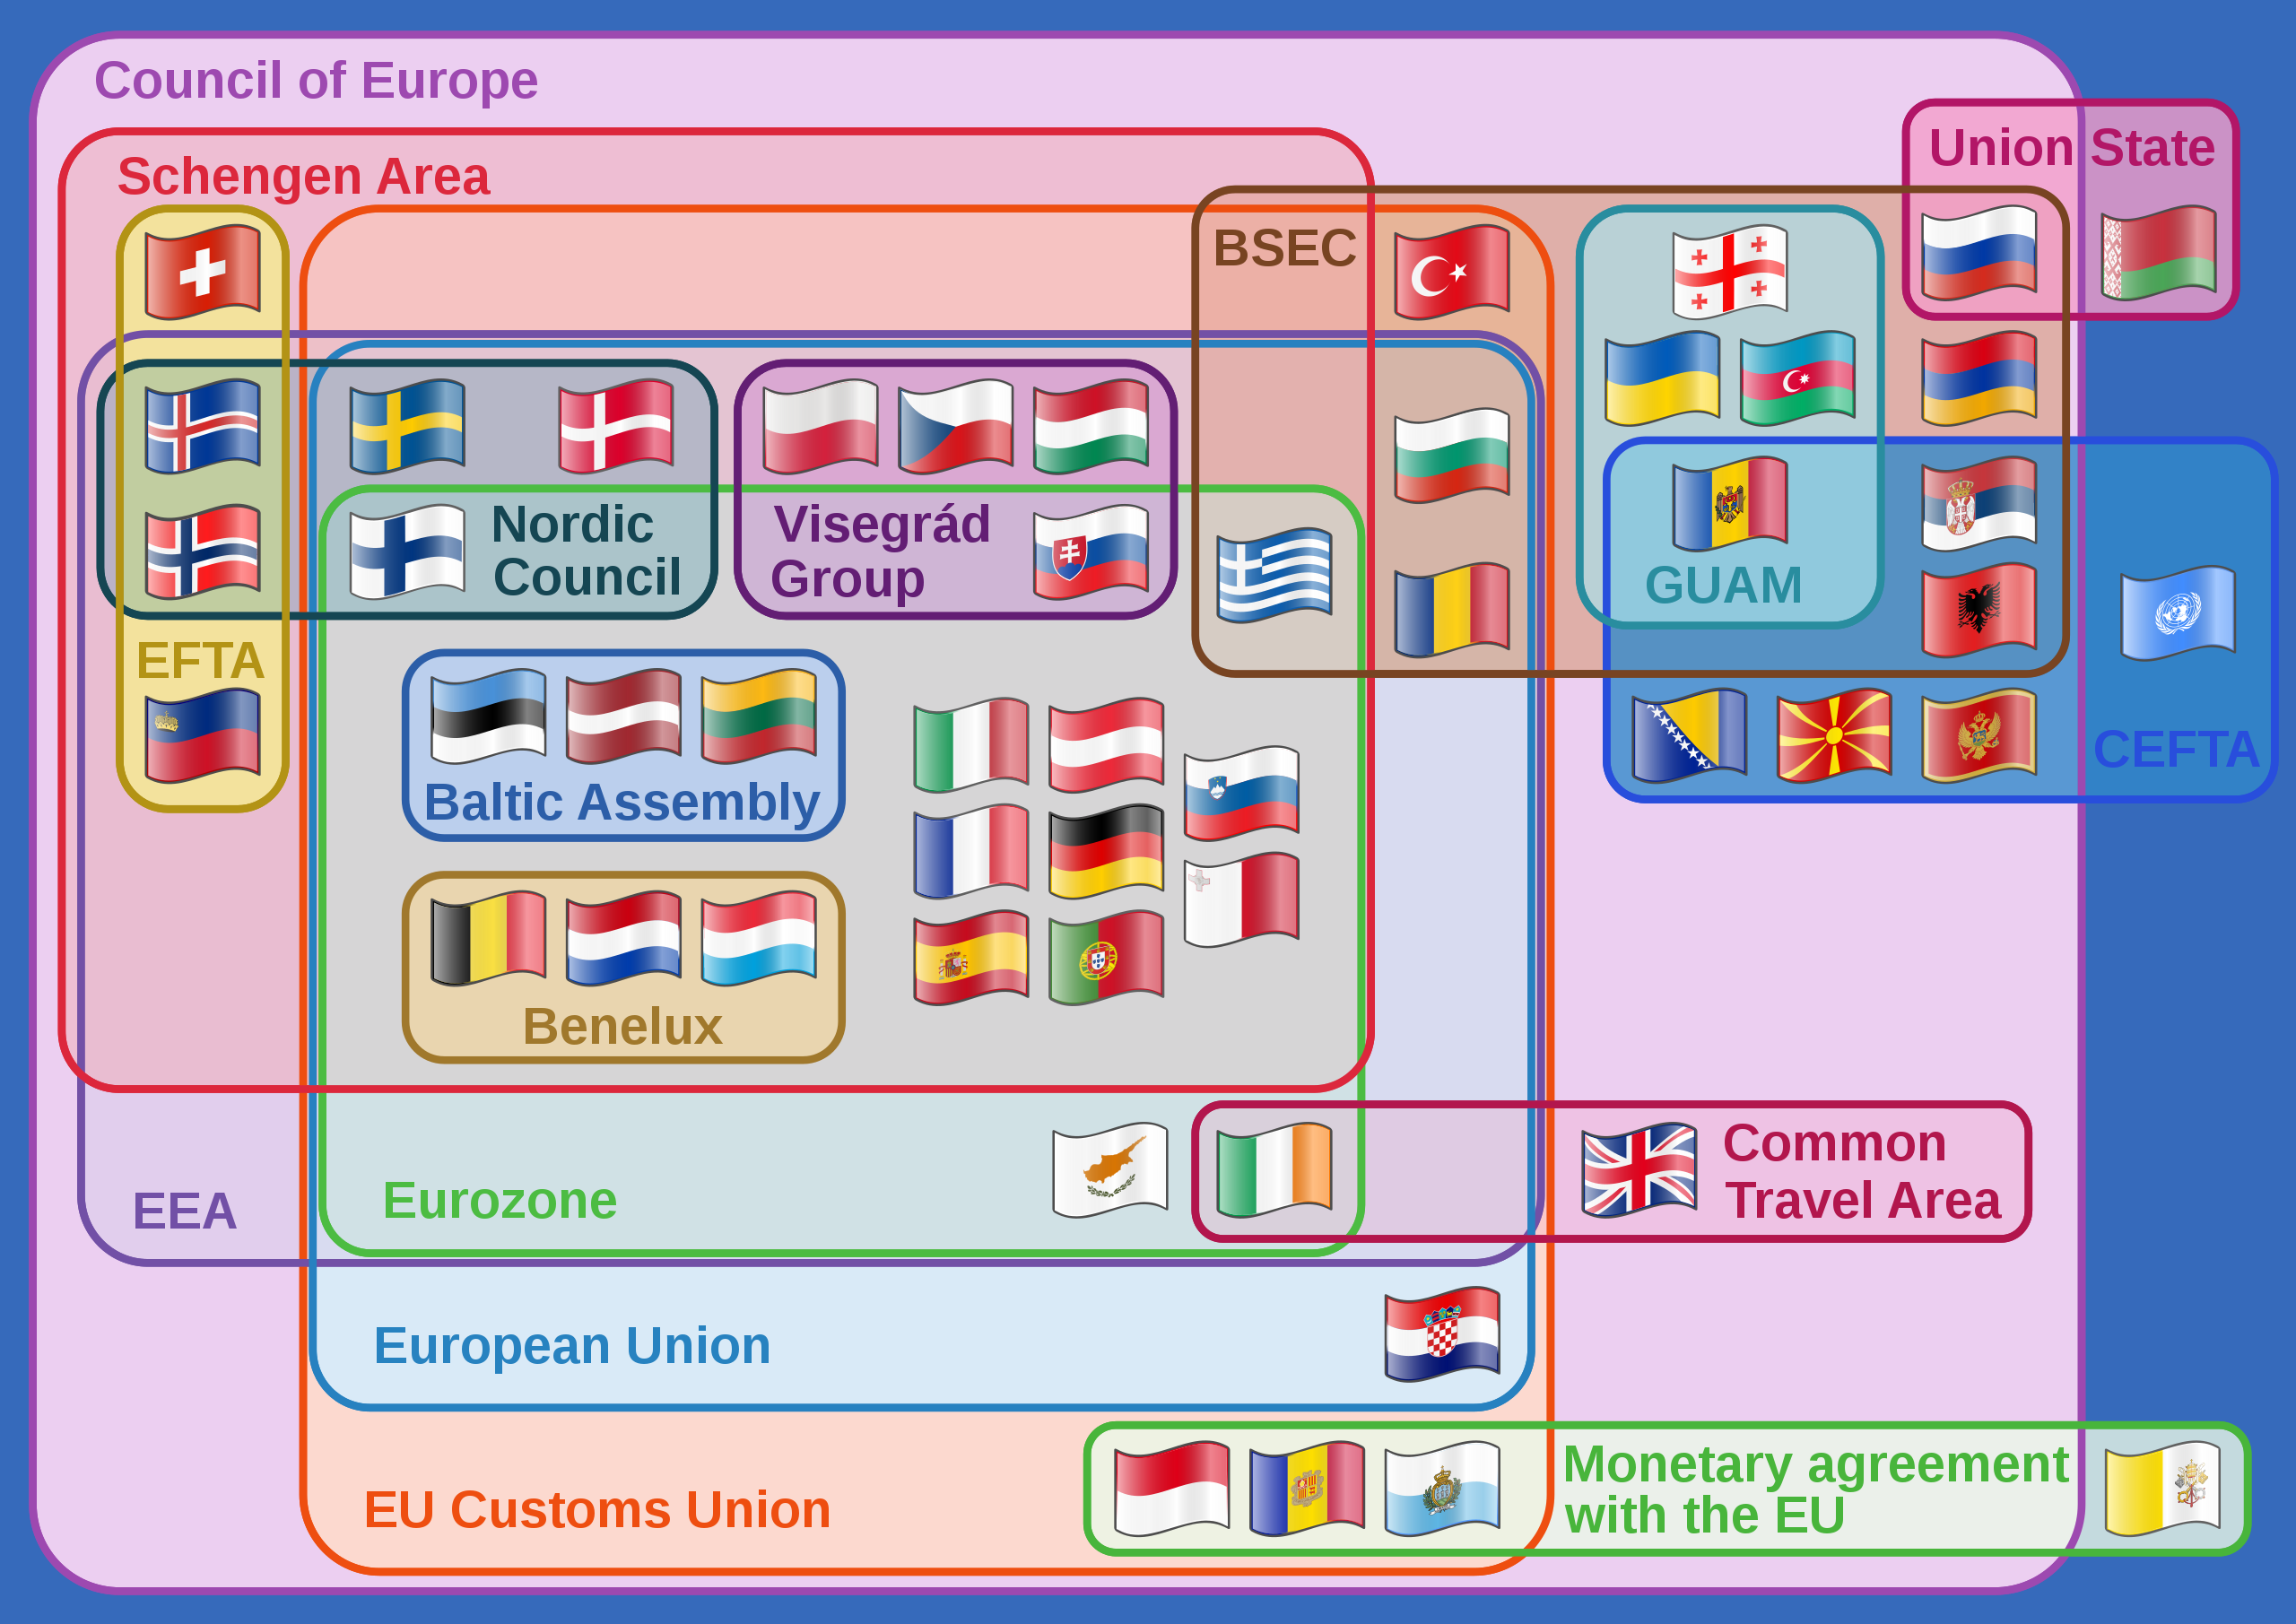
\includegraphics[width=0.7\linewidth]{../figures/europe-groups}
	\caption{Euler Diagram illustrating the various multinational European organizations and agreements. European Union is shown in light blue; EEA is in purple. Source: \href{https://en.wikipedia.org/wiki/File:Supranational_European_Bodies-en.svg}{Wikipedia}
	}
	\label{fig:europe-groups}
\end{figure}
.

\section{References}


\end{document}